% !TeX program = xelatex
\documentclass[a4paper,10pt]{article}

% ============================================================================
% កិច្ចតែងការបង្រៀនមុខវិជ្ជាគណិតវិទ្យា ថ្នាក់ទី៨ (ម៉ោងសិក្សា ៥០ នាទី — គ្មាន LCD / ប្រើសន្លឹកកិច្ចការជាគោល)
% មេរៀនទី១៧៖ រូបធរណីមាត្រដែលមានវិមាត្របី | ម៉ោងទី៦ (១៧.៤)៖ ការគណនាមាឌនៃកោន និងលំហាត់សំយោគ (ទំ.២២៥–២៣០)
% វិធីសាស្ត្រ៖ Erroneous Slant-Height Diagnosis (h vs s) + Composite 3D Engineering & Backward-Formula Synthesis Worksheet
% ============================================================================
\usepackage[a4paper, left=0.95cm, right=0.95cm, top=0.85cm, bottom=0.92cm, footskip=0.52cm]{geometry}
\usepackage{amsmath}
\usepackage{unicode-math}
\usepackage{fontspec}
\usepackage{longtable, array, multirow, colortbl}
\usepackage[table]{xcolor}
\usepackage{enumitem}
\usepackage{pifont}
\usepackage{fancyhdr}
\usepackage{tikz}
\usetikzlibrary{calc, arrows.meta, angles, quotes, patterns, decorations.markings, babel}

\makeatletter
\let\@expl@@@mark@update@singlecol@structures@@\relax
\makeatother

% -------------------- ការស្វែងរកទីតាំងពុម្ពអក្សរដោយស្វ័យប្រវត្តិ (\NGSFindFonts) --------------------
\providecommand{\NGSFindFonts}{%
  \IfFileExists{C:/Windows/Fonts/cambria.ttc}{%
    \def\NGSSysPath{C:/Windows/Fonts/}%
    \def\NGSUserPath{C:/Users/KIT/AppData/Local/Microsoft/Windows/Fonts/}%
  }{%
    \IfFileExists{./fonts/KhmerOSsiemreap.ttf}{\def\NGSSysPath{./fonts/}\def\NGSUserPath{./fonts/}}{%
    \IfFileExists{../fonts/KhmerOSsiemreap.ttf}{\def\NGSSysPath{../fonts/}\def\NGSUserPath{../fonts/}}{%
    \IfFileExists{../../fonts/KhmerOSsiemreap.ttf}{\def\NGSSysPath{../../fonts/}\def\NGSUserPath{../../fonts/}}{%
    \IfFileExists{../../../fonts/KhmerOSsiemreap.ttf}{\def\NGSSysPath{../../../fonts/}\def\NGSUserPath{../../../fonts/}}{%
    \IfFileExists{../../../../fonts/KhmerOSsiemreap.ttf}{\def\NGSSysPath{../../../../fonts/}\def\NGSUserPath{../../../../fonts/}}{%
    \IfFileExists{../../../../../fonts/KhmerOSsiemreap.ttf}{\def\NGSSysPath{../../../../../fonts/}\def\NGSUserPath{../../../../../fonts/}}{%
    \IfFileExists{../../../../../../fonts/KhmerOSsiemreap.ttf}{\def\NGSSysPath{../../../../../../fonts/}\def\NGSUserPath{../../../../../../fonts/}}{%
      \def\NGSSysPath{../../../../../../../fonts/}\def\NGSUserPath{../../../../../../../fonts/}%
    }}}}}}}%
  }%
}
\NGSFindFonts

\setmathfont[Path={\NGSSysPath}, FontIndex=1, Scale=1.02]{cambria.ttc}
\defaultfontfeatures{Ligatures=TeX}

\setmainfont[
  Path={\NGSUserPath},
  Extension=.ttf,
  Script=Khmer,
  BoldFont={KhmerOSsiemreap},
  BoldFeatures={FakeBold=1.8},
  ItalicFont={KhmerOSsiemreap},
  ItalicFeatures={FakeSlant=0.25},
  BoldItalicFont={KhmerOSsiemreap},
  BoldItalicFeatures={FakeBold=1.8, FakeSlant=0.25}
]{KhmerOSsiemreap}

\newfontfamily\muol[
  Path={\NGSUserPath},
  Extension=.ttf,
  Script=Khmer
]{KhmerOSmuollight}

\newfontfamily\NagaBold[
  Path={\NGSUserPath},
  Extension=.ttf,
  Script=Khmer,
  ItalicFont={AKbalthom Naga Bold},
  ItalicFeatures={FakeSlant=0.22}
]{AKbalthom Naga Bold}

\newfontfamily\Tacteing[
  Path={\NGSUserPath},
  Extension=.TTF
]{TACTENG}

\newfontfamily\CalibriPage[
  Path={\NGSSysPath},
  Extension=.ttf
]{calibri}

\newfontfamily\TimesEn[
  Path={\NGSSysPath},
  Extension=.ttf,
  BoldFont={timesbd},
  ItalicFont={timesi},
  BoldItalicFont={timesbi}
]{times}

\newfontfamily\SymbolCirc[
  Path={\NGSSysPath},
  Extension=.ttf
]{cour}
\newcommand{\wcirc}{{\SymbolCirc\fontsize{10.5pt}{12pt}\selectfont o}}

\XeTeXlinebreaklocale "km"
\XeTeXlinebreakskip = 0pt plus 1pt minus 0.1pt

% -------------------- ពណ៌ និងការតុបតែង --------------------
\definecolor{darkred}{RGB}{180, 0, 0}
\definecolor{red5e}{RGB}{210, 15, 15}
\definecolor{headgray}{gray}{0.86}
\definecolor{stepgray}{gray}{0.91}
\definecolor{boxgray}{gray}{0.93}

\pagestyle{fancy}
\fancyhf{}
\renewcommand{\headrulewidth}{0pt}
\fancyfoot[R]{{\CalibriPage\fontsize{9.5pt}{11pt}\selectfont \thepage}}

\setlength{\parindent}{0pt}
\setlength{\parskip}{0pt}
\setlength{\LTpre}{2pt}
\setlength{\LTpost}{2pt}
\setlength{\tabcolsep}{4.5pt}
\arrayrulewidth=0.45pt

\newcolumntype{L}[1]{>{\raggedright\arraybackslash}p{#1}}
\newcolumntype{C}[1]{>{\centering\arraybackslash}p{#1}}

\newcommand{\en}[1]{{\TimesEn #1}}
\newcommand{\enbf}[1]{{\TimesEn\textbf{#1}}}
\newcommand{\unit}[1]{\,\text{\en{#1}}}
\newcommand{\fiveE}[1]{{\NagaBold\fontsize{9.5pt}{13pt}\selectfont\textcolor{red5e}{#1}}}
\newcommand{\timenote}[1]{\textcolor{darkred}{\textit{#1}}}
\newcommand{\khmflourish}{{\Tacteing\fontsize{17pt}{17pt}\selectfont 3}}
\newcommand{\graybox}[1]{\colorbox{boxgray}{\strut\hspace{2pt}#1\hspace{2pt}}}
\newcommand{\ditem}{\tikz[baseline=-0.5ex]\fill (0,0.42ex) -- (0.42ex,0) -- (0,-0.42ex) -- (-0.42ex,0) -- cycle;\hspace{0.3em}}
\newcommand{\cnum}[1]{{\fontsize{10.5pt}{12pt}\selectfont\ding{\numexpr181+#1\relax}}\hspace{0.2em}}
\newcommand{\cfig}[1]{\par\vspace{4pt}{\centering #1\par}\vspace{4pt}}
\newcommand{\stepheader}[1]{\multicolumn{3}{|c|}{\cellcolor{stepgray}\muol #1} \\* \noalign{\hrule height 0.4pt}}
\newcommand{\tri}[1]{\ensuremath{\triangle #1}}

\newcommand{\rightbox}[4][0.18]{%
  \draw[black, line width=0.75pt]
    ($(#3)!#1!(#2)$) -- ($($(#3)!#1!(#2)$)+($(#3)!#1!(#4)$)-(#3)$) -- ($(#3)!#1!(#4)$);
}

% ============================================================================
% រូបធរណីមាត្រ ស-ខ្មៅ (B&W Print-Safe TikZ Figures for Hour 17.6: Cone Volume & Synthesis)
% ============================================================================

% ១. កំណែកិច្ចការផ្ទះទី២១ (ទំ.២៣០) និងរំលឹកត្រីកោណកែងកំណើតកោន (r, h, s)
\newcommand{\figPrereqConeVol}{%
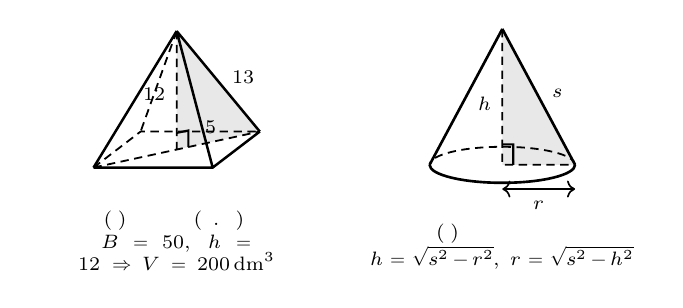
\begin{tikzpicture}[scale=0.88, every node/.style={font=\scriptsize, text=black}]
  % (ក) លំហាត់ទី២១ (ទំ.២៣០)៖ ពីរ៉ាមីតបាតការេ អង្កត់ទ្រូងបាត 10dm (កន្លះ=5dm), ទ្រនុងខាង 13dm => h=12dm
  \begin{scope}[shift={(-2.35,0)}]
    \coordinate (V) at (0,1.25);
    \coordinate (A) at (-1.20,-0.72);
    \coordinate (B) at (0.52,-0.72);
    \coordinate (C) at (1.20,-0.20);
    \coordinate (D) at (-0.52,-0.20);
    \coordinate (O) at (0,-0.46);
    \fill[gray!18] (V) -- (O) -- (C) -- cycle;
    \draw[black, line width=0.9pt] (A) -- (B) -- (C) (V) -- (A) (V) -- (B) (V) -- (C);
    \draw[black, line width=0.65pt, densely dashed] (A) -- (D) -- (C) (V) -- (D) (A) -- (C) (V) -- (O);
    \rightbox[0.14]{V}{O}{C}
    \node[left=0.5pt] at (0,0.34) {$12$};
    \node[above left=-1.5pt] at (0.66,-0.31) {$5$};
    \node[right=1pt] at (0.62,0.58) {$13$};
    \node[align=center, text width=3.55cm] at (0.0,-1.78) {(ក) លំហាត់ទី២១ (ទំ.២៣០)៖\\$B=50,\; h=12 \Rightarrow V=200\unit{dm}^3$};
  \end{scope}

  % (ខ) រំលឹកត្រីកោណកែងកំណើតកោន (h^2 + r^2 = s^2)
  \begin{scope}[shift={(2.35,0)}]
    \coordinate (V) at (0,1.28);
    \coordinate (O) at (0,-0.68);
    \coordinate (L) at (-1.05,-0.68);
    \coordinate (R) at (1.05,-0.68);
    \fill[gray!18] (V) -- (O) -- (R) -- cycle;
    \draw[black, line width=0.95pt] (L) arc (-180:0:1.05 and 0.26) (V) -- (L) (V) -- (R);
    \draw[black, line width=0.65pt, densely dashed] (R) arc (0:180:1.05 and 0.26) (V) -- (O) -- (R);
    \rightbox[0.15]{V}{O}{R}
    \node[left=0.5pt] at (0,0.20) {$h$};
    \draw[<->, line width=0.6pt] (0,-1.03) -- (1.05,-1.03) node[midway, below=0.5pt] {$r$};
    \node[right=1pt] at (0.55,0.35) {$s$};
    \node[align=center, text width=3.65cm] at (0.0,-1.86) {(ខ) ត្រីកោណកែងក្នុងកោន៖\\$h = \sqrt{s^2 - r^2},\; r = \sqrt{s^2 - h^2}$};
  \end{scope}
\end{tikzpicture}}

% ២. E1 Engage (លំហាត់ទី១៨ ទំ.២២៩)៖ អណ្ដូងទឹករាងស៊ីឡាំងជម្រៅ 50m (d=6m => r=3m) + បាតកោនជនេត្រ s=5m
\newcommand{\figEngageWell}{%
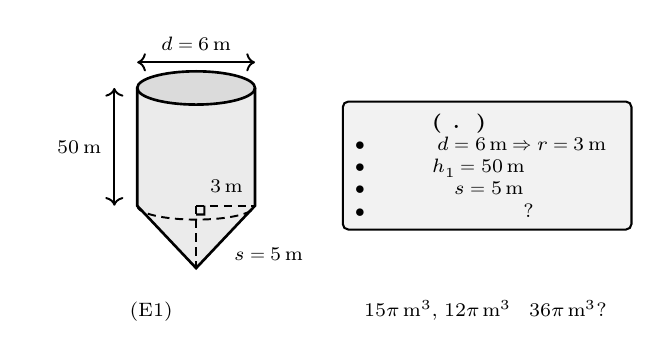
\begin{tikzpicture}[scale=0.88, every node/.style={font=\scriptsize, text=black}]
  \begin{scope}[shift={(-1.65,0.05)}]
    \fill[gray!16] (-0.85,-0.55) -- (-0.85,1.15) arc (180:360:0.85 and 0.24) -- (0.85,-0.55) -- (0,-1.45) -- cycle;
    \fill[gray!28] (0,1.15) ellipse (0.85 and 0.24);
    \draw[black, line width=0.95pt] (0,1.15) ellipse (0.85 and 0.24);
    \draw[black, line width=0.95pt] (-0.85,1.15) -- (-0.85,-0.55) -- (0,-1.45) -- (0.85,-0.55) -- (0.85,1.15);
    \draw[black, line width=0.70pt, densely dashed] (-0.85,-0.55) arc (-180:0:0.85 and 0.20);
    \draw[black, line width=0.75pt, densely dashed] (0,-0.55) -- (0,-1.45) (0,-0.55) -- (0.85,-0.55);
    \rightbox[0.14]{0,-1.45}{0,-0.55}{0.85,-0.55}
    \draw[<->, line width=0.7pt] (-0.85,1.52) -- (0.85,1.52) node[midway, above=0.5pt] {$d = 6\unit{m}$};
    \draw[<->, line width=0.7pt] (-1.18,-0.55) -- (-1.18,1.15) node[midway, left=1pt] {$50\unit{m}$};
    \node[below right=-1pt] at (0.45,-1.05) {$s = 5\unit{m}$};
    \node[above=1pt] at (0.44,-0.55) {$3\unit{m}$};
  \end{scope}

  \begin{scope}[shift={(2.25,0.08)}]
    \node[draw=black, line width=0.75pt, rounded corners=2pt, fill=gray!10, inner sep=4.5pt, align=left, text width=3.35cm] at (0.30,0.0) {%
      \textbf{អណ្ដូងទឹកទី១៨ (ទំ.២២៩)៖}\\
      $\bullet$ មាត់អណ្ដូង៖ $d=6\unit{m}\Rightarrow r=3\unit{m}$\\
      $\bullet$ តួស៊ីឡាំង៖ $h_1 = 50\unit{m}$\\
      $\bullet$ បាតកោន៖ ជនេត្រ $s = 5\unit{m}$\\
      $\bullet$ តើមាឌផ្នែកបាតកោនស្មើប៉ុន្មាន?};
  \end{scope}
  \node[align=center, text width=7.3cm] at (0.20,-2.02) {បញ្ហាបំផុសគំនិត (\en{E1})៖ តើបាតរាងកោនខាងក្រោមមានមាឌស្មើនឹង $15\pi\unit{m}^3$, $12\pi\unit{m}^3$ ឬ $36\pi\unit{m}^3$?};
\end{tikzpicture}}

% ៣. E2/E3 ការផ្ទេរ ៣ ដងពីកោនចូលស៊ីឡាំង (ទំ.២២៥) និងលំហាត់គំរូទី 2 (r=6, s=10 => h=8, V=301.4)
\newcommand{\figCylConeAndExTwo}{%
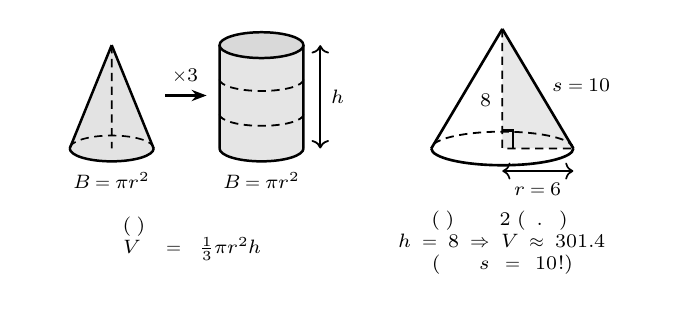
\begin{tikzpicture}[scale=0.82, every node/.style={font=\scriptsize, text=black}]
  % (ក) កោន x 3 = ស៊ីឡាំង (បាតថាសកាំ r និងកម្ពស់ h ស្មើគ្នា)
  \begin{scope}[shift={(-2.50,0)}]
    \coordinate (V) at (-0.95,0.88);
    \coordinate (L) at (-1.60,-0.72);
    \coordinate (R) at (-0.30,-0.72);
    \fill[gray!22] (L) -- (V) -- (R) arc (0:-180:0.65 and 0.20);
    \draw[black, line width=0.9pt] (L) arc (-180:0:0.65 and 0.20) (V) -- (L) (V) -- (R);
    \draw[black, line width=0.6pt, densely dashed] (R) arc (0:180:0.65 and 0.20) (V) -- (-0.95,-0.72);
    \node[below=1pt] at (-0.95,-0.90) {$B=\pi r^2$};

    \draw[-{Stealth[length=1.9mm]}, line width=0.85pt] (-0.12,0.10) -- (0.52,0.10) node[midway, above=1pt] {$\times 3$};

    \fill[gray!20] (0.72,-0.72) -- (0.72,0.88) arc (180:360:0.65 and 0.20) -- (2.02,-0.72) arc (0:-180:0.65 and 0.20);
    \fill[gray!30] (1.37,0.88) ellipse (0.65 and 0.20);
    \draw[black, line width=0.65pt, densely dashed] (0.72,-0.19) arc (-180:0:0.65 and 0.18) (0.72,0.35) arc (-180:0:0.65 and 0.18);
    \draw[black, line width=0.9pt] (1.37,0.88) ellipse (0.65 and 0.20);
    \draw[black, line width=0.9pt] (0.72,-0.72) -- (0.72,0.88) (2.02,-0.72) -- (2.02,0.88) (0.72,-0.72) arc (-180:0:0.65 and 0.20);
    \draw[<->, line width=0.65pt] (2.28,-0.72) -- (2.28,0.88) node[midway, right=0.5pt] {$h$};
    \node[below=1pt] at (1.37,-0.90) {$B=\pi r^2$};
    \node[align=center, text width=3.95cm] at (0.30,-2.12) {(ក) ចាក់ ៣ ដងពេញស៊ីឡាំង៖\\$V_{\text{កោន}} = \frac{1}{3}\pi r^2 h$};
  \end{scope}

  % (ខ) លំហាត់គំរូទី 2 (ទំ.២២៦)៖ កោន r=6, s=10 => h=8
  \begin{scope}[shift={(2.60,-0.02)}]
    \coordinate (V) at (0,1.15);
    \coordinate (O) at (0,-0.70);
    \coordinate (L) at (-1.10,-0.70);
    \coordinate (R) at (1.10,-0.70);
    \fill[gray!18] (V) -- (O) -- (R) -- cycle;
    \draw[black, line width=0.95pt] (L) arc (-180:0:1.10 and 0.26) (V) -- (L) (V) -- (R);
    \draw[black, line width=0.65pt, densely dashed] (R) arc (0:180:1.10 and 0.26) (V) -- (O) -- (R);
    \rightbox[0.15]{V}{O}{R}
    \node[left=0.5pt] at (0,0.05) {$8$};
    \draw[<->, line width=0.6pt] (0,-1.05) -- (1.10,-1.05) node[midway, below=0.5pt] {$r=6$};
    \node[right=1pt] at (0.58,0.28) {$s=10$};
    \node[align=center, text width=3.65cm] at (0.0,-2.16) {(ខ) គំរូទី \en{2} (ទំ.២២៦)៖\\$h=8 \Rightarrow V\approx 301.4$ (មិនមែន $s=10$!)};
  \end{scope}
\end{tikzpicture}}

% ៤. E4 ប្រតិបត្តិ ក (r=3, h=6 => V=56.52) និង ប្រតិបត្តិ ខ (h=5, s=13 => r=12, V=753.6) ទំ.២២៦
\newcommand{\figElaborateConeVol}{%
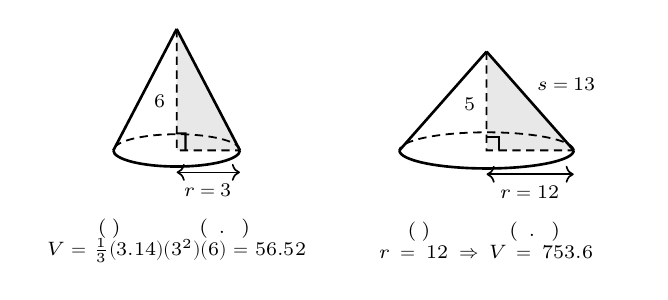
\begin{tikzpicture}[scale=0.82, every node/.style={font=\scriptsize, text=black}]
  % (១) ប្រតិបត្តិ ក (ទំ.២២៦)៖ r=3, h=6
  \begin{scope}[shift={(-2.35,0)}]
    \coordinate (V) at (0,1.20);
    \coordinate (O) at (0,-0.68);
    \coordinate (L) at (-0.98,-0.68);
    \coordinate (R) at (0.98,-0.68);
    \fill[gray!18] (V) -- (O) -- (R) -- cycle;
    \draw[black, line width=0.95pt] (L) arc (-180:0:0.98 and 0.25) (V) -- (L) (V) -- (R);
    \draw[black, line width=0.65pt, densely dashed] (R) arc (0:180:0.98 and 0.25) (V) -- (O) -- (R);
    \rightbox[0.14]{V}{O}{R}
    \node[left=0.5pt] at (0,0.08) {$6$};
    \draw[<->, line width=0.6pt] (0,-1.02) -- (0.98,-1.02) node[midway, below=0.5pt] {$r=3$};
    \node[align=center, text width=3.55cm] at (0.0,-2.08) {(១) ប្រតិបត្តិ ក (ទំ.២២៦)៖\\$V = \frac{1}{3}(3.14)(3^2)(6) = 56.52$};
  \end{scope}

  % (២) ប្រតិបត្តិ ខ (ទំ.២២៦)៖ h=5, s=13 => r=12
  \begin{scope}[shift={(2.45,0)}]
    \coordinate (V) at (0,0.85);
    \coordinate (O) at (0,-0.68);
    \coordinate (L) at (-1.35,-0.68);
    \coordinate (R) at (1.35,-0.68);
    \fill[gray!18] (V) -- (O) -- (R) -- cycle;
    \draw[black, line width=0.95pt] (L) arc (-180:0:1.35 and 0.28) (V) -- (L) (V) -- (R);
    \draw[black, line width=0.65pt, densely dashed] (R) arc (0:180:1.35 and 0.28) (V) -- (O) -- (R);
    \rightbox[0.14]{V}{O}{R}
    \node[left=0.5pt] at (0,0.04) {$5$};
    \draw[<->, line width=0.6pt] (0,-1.05) -- (1.35,-1.05) node[midway, below=0.5pt] {$r=12$};
    \node[above right=-1pt] at (0.68,0.14) {$s=13$};
    \node[align=center, text width=3.65cm] at (0.0,-2.08) {(២) ប្រតិបត្តិ ខ (ទំ.២២៦)៖\\$r=12 \Rightarrow V = 753.6$};
  \end{scope}
\end{tikzpicture}}

% ============================================================================
% ចាប់ផ្ដើមឯកសារ (Document Body)
% ============================================================================
\begin{document}
\fontsize{10pt}{15.2pt}\selectfont

% -------------------- ក្បាលកិច្ចតែងការ (Header) --------------------
\begin{center}
  {\muol\fontsize{11pt}{16pt}\selectfont ព្រះរាជាណាចក្រកម្ពុជា}\\[2pt]
  {\muol\fontsize{10pt}{15pt}\selectfont ជាតិ សាសនា ព្រះមហាក្សត្រ}\\[1pt]
  \khmflourish
\end{center}

\vspace{-26pt}
{\muol\fontsize{9.5pt}{12.8pt}\selectfont
មន្ទីរអប់រំ យុវជន និងកីឡា ខេត្តកំពង់ធំ\\
ការិយាល័យអប់រំ យុវជន និងកីឡា ស្រុកកំពង់ស្វាយ\\
អនុវិទ្យាល័យព្រះក្រសាំង}

\vspace{2pt}
\begin{center}
  {\muol\fontsize{10pt}{14.5pt}\selectfont កិច្ចតែងការបង្រៀន}
\end{center}
\vspace{1pt}

% -------------------- ព័ត៌មានទូទៅ (Metadata) --------------------
{\renewcommand{\arraystretch}{0.98}
\hspace*{4.05cm}%
\begin{tabular}{@{}l l l@{}}
  - \hspace{0.35cm} មុខវិជ្ជា & : & គណិតវិទ្យា ថ្នាក់ទី៨ \\
  - \hspace{0.35cm} ចំណងជើងមេរៀន & : & មេរៀនទី១៧ រូបធរណីមាត្រដែលមានវិមាត្របី \\
  - \hspace{0.35cm} ចំណងជើងរង & : & ១៧.៤ ការគណនាមាឌនៃកោន និងលំហាត់សំយោគ (ទំព័រ ២២៥--២៣០) \\
  - \hspace{0.35cm} រយៈពេល & : & ១ ម៉ោងសិក្សា (៥០ នាទី) \\
  - \hspace{0.35cm} បង្រៀនដោយ & : & ហុក ប៊ុនថែន \\
  - \hspace{0.35cm} កាលបរិច្ឆេទ & : & ថ្ងៃ\makebox[18mm]{\dotfill}\ ទី\makebox[8mm]{\dotfill}\ ខែ\makebox[18mm]{\dotfill}\ ឆ្នាំ២០២៦ \\
\end{tabular}

\vspace{3pt}

% -------------------- I. វត្ថុបំណង --------------------
\textbf{I.} {\muol វត្ថុបំណង}\\[1pt]
\hspace*{0.55cm}%
\begin{tabular}{@{}l l L{14.2cm}@{}}
  \wcirc \hspace{0.25cm} វិជ្ជាសម្បទា & : & សិស្សប្រាប់បានត្រឹមត្រូវពីរូបមន្តគណនាមាឌនៃកោន ($V = \frac{1}{3}B\cdot h = \frac{1}{3}\pi r^2 h$) និងសំយោគប្រៀបធៀបរូបមន្តមាឌនៃសូលីតទាំង ៤ (ព្រីស ស៊ីឡាំង ពីរ៉ាមីត និងកោន) ។ \\
  \wcirc \hspace{0.25cm} បំណិនសម្បទា & : & សិស្សវិភាគរកកំហុសនៃការជំនួសជនេត្រ $s$ ជំនួសកម្ពស់កែង $h$ ប្រើពីតាកររកធាតុបាត់ ($h$ ឬ $r$) ទាញបញ្ច្រាសរូបមន្តរក $B$ ឬ $h$ ពីមាឌ $V$ និងដោះស្រាយបញ្ហាសូលីតផ្សំលើសន្លឹកកិច្ចការបានត្រឹមត្រូវ ។ \\
  \wcirc \hspace{0.25cm} ចរិយាសម្បទា & : & សិស្សមានស្មារតីត្រិះរិះពិចារណាផ្ទៀងផ្ទាត់ទិន្នន័យធរណីមាត្រ និងឱ្យតម្លៃលើការអនុវត្តរូបមន្តសូលីតក្នុងវិស្វកម្មជីវភាពពិត ។ \\
\end{tabular}

\vspace{3pt}

% -------------------- II. សម្ភារៈឧបទេស --------------------
\textbf{II.} {\muol សម្ភារៈឧបទេស}\\[1pt]
\hspace*{0.55cm}$\bullet$ \hspace{0.35cm} សៀវភៅសិក្សាគោលគណិតវិទ្យាថ្នាក់ទី៨ (ទំ.២២៥--២៣០) សន្លឹកកិច្ចការសិស្ស ស-ខ្មៅ (\en{Worksheet\_CONE\_VOL} ចំនួន ២ ទំព័រ គ្មាន \en{LCD}) ក្ដារខៀន ដីស និងបន្ទាត់ក្រិត ។

\vspace{3pt}

% -------------------- III. វិធីសាស្រ្តបង្រៀន --------------------
\textbf{III.} {\muol វិធីសាស្រ្តបង្រៀន}\\[1pt]
\hspace*{0.45cm}%
\begin{tabular}{@{}l l L{14.85cm}@{}}
  $\bullet$ \hspace{0.25cm} គោលវិធី & : & សិស្សមជ្ឈមណ្ឌល (សិក្សាតាមរយៈការបំពេញលើសន្លឹកកិច្ចការជាគោល គ្មាន \en{LCD} និងគ្មានការកាត់បិទក្រដាស) \\
  $\bullet$ \hspace{0.25cm} យុទ្ធវិធីបង្រៀន & : & ស្ថាបនានិយម គម្រូ \en{5Es} រួមបញ្ចូលការវិភាគកំហុសជនេត្រទល់កម្ពស់កែង (\en{Erroneous Slant-Height Diagnosis}) ការទាញបញ្ច្រាសរូបមន្ត និងការដោះស្រាយបញ្ហាសូលីតផ្សំ ។ \\
\end{tabular}
}

\vspace{3pt}

% -------------------- IV. ដំណើរការបង្រៀន --------------------
\textbf{IV.} {\muol ដំណើរការបង្រៀន}

\vspace{2pt}

\renewcommand{\arraystretch}{1.15}
\begin{longtable}{|L{5.50cm}|L{7.90cm}|L{4.80cm}|}
\hline
\rowcolor{headgray}
\multicolumn{1}{|c|}{\muol សកម្មភាពគ្រូ} &
\multicolumn{1}{c|}{\muol ខ្លឹមសារមេរៀន} &
\multicolumn{1}{c|}{\muol សកម្មភាពសិស្ស} \\
\hline
\endfirsthead

\hline
\rowcolor{headgray}
\multicolumn{1}{|c|}{\muol សកម្មភាពគ្រូ} &
\multicolumn{1}{c|}{\muol ខ្លឹមសារមេរៀន} &
\multicolumn{1}{c|}{\muol សកម្មភាពសិស្ស} \\
\hline
\endhead

\hline
\endfoot

\hline
\endlastfoot

% ==================== ជំហានទី១ (2 min) ====================
\stepheader{ជំហានទី១ (រដ្ឋបាលថ្នាក់)}
$\bullet$ ពិនិត្យវត្តមាន សណ្ដាប់ធ្នាប់ អនាម័យ និងចែកសន្លឹកកិច្ចការ \en{Worksheet\_CONE\_VOL} ដល់សិស្សគ្រប់គូ \timenote{(2 min)}
&
$\bullet$ រដ្ឋបាលថ្នាក់ និងការត្រៀមសៀវភៅគោល បន្ទាត់ក្រិត និងសន្លឹកកិច្ចការសិស្ស
&
$\circ$ ប្រធានថ្នាក់រាយការណ៍វត្តមាន\par\vspace{2pt}
$\circ$ ទទួលសន្លឹកកិច្ចការ និងត្រៀមឧបករណ៍ \\[3pt]
\hline

% ==================== ជំហានទី២ (9 min: ≤3 + 3 + E1 3) ====================
\stepheader{ជំហានទី២ (កិច្ចការផ្ទះ + រំលឹកមេរៀនចាស់ + ទំនាក់ទំនងមេរៀនថ្មី)}
\timenote{(កំណែកិច្ចការផ្ទះ $\le 3\text{ min}$)}\par\vspace{1pt}
$\bullet$ ផ្ទៀងផ្ទាត់ចម្លើយលំហាត់ទី៨ង (ទំ.២២៨) និងលំហាត់ទី២១ (ទំ.២៣០) លើក្ដារខៀនយ៉ាងរហ័ស
&
\textbf{កំណែកិច្ចការផ្ទះ (ទំ.២២៨ ទី៨ង និងទំ.២៣០ ទី២១)៖}\par\vspace{1pt}
$1.$ \textbf{ទី៨ង៖} $V = 20^3 + \frac{1}{3}(20^2)(15) = 8000 + 2000 = \mathbf{10\,000\unit{ft}^3}$ ។\par\vspace{1pt}
$2.$ \textbf{ទី២១៖} $B = \frac{10^2}{2} = 50\unit{dm}^2$,\; $h = \sqrt{13^2-5^2} = 12\unit{dm} \Rightarrow V = \frac{1}{3}(50)(12) = \graybox{$200\unit{dm}^3$}$ ។
&
$\circ$ ផ្ទៀងផ្ទាត់និងកែកំណែលំហាត់ទី៨ង និងទី២១ ក្នុងសៀវភៅ \\[3pt]

\timenote{(រំលឹកមេរៀនចាស់ 3 min)}\par\vspace{1pt}
$\bullet$ សួររំលឹករូបមន្តមាឌស៊ីឡាំង និងមាឌពីរ៉ាមីតដែលបានរៀនម៉ោងមុន
&
\textbf{រំលឹកមាឌស៊ីឡាំង មាឌពីរ៉ាមីត និងត្រីកោណកែងកំណើតកោន៖}\par\vspace{1pt}
\ditem ស៊ីឡាំង៖ $V = \pi r^2 h$ \;\textbar\; ពីរ៉ាមីត៖ $V = \dfrac{1}{3}B\cdot h$ ។
&
$\circ$ ឆ្លើយរំលឹករូបមន្តមាឌស៊ីឡាំង និងមាឌពីរ៉ាមីត \\[3pt]

$\bullet$ សួរ៖ «ក្នុងកោនបរិវត្ត តើកាំ $r$ កម្ពស់កែង $h$ និងជនេត្រ $s$ ទាក់ទងគ្នាតាមសមីការអ្វី?»
&
\ditem ត្រីកោណកែងក្នុងកោន៖ $h^2 + r^2 = s^2 \Rightarrow h = \sqrt{s^2-r^2}$ ។
&
$\circ$ ឆ្លើយទំនាក់ទំនងពីតាករ $h = \sqrt{s^2-r^2}$ \\[3pt]

& \cfig{\figPrereqConeVol} & \\[3pt]

\fiveE{E1 - Engage} \timenote{(3 min)}\par\vspace{1.5pt}
$\bullet$ បង្ហាញបញ្ហាជីកអណ្ដូងទឹកលើ \textbf{បេសកកម្មទី១ (\en{E1})} (ដកស្រង់ពីលំហាត់ទី១៨ ទំ.២២៩)៖\par\vspace{1pt}
\hspace*{0.3em}-- «អណ្ដូងទឹកមួយមានតួលើរាងស៊ីឡាំងអង្កត់ផ្ចិតមាត់ $d = 6\unit{m}$ ជម្រៅ $50\unit{m}$ និងបាតក្រោមរាងកោនដែលមានជនេត្រទ្រេត $s = 5\unit{m}$ ។ តើផ្នែកបាតរាងកោនខាងក្រោមមានមាឌស្មើនឹង $15\pi\unit{m}^3$, $12\pi\unit{m}^3$ ឬ $36\pi\unit{m}^3$?»
&
\textbf{១៧.៤ ការគណនាមាឌនៃកោន និងលំហាត់សំយោគ}\par\vspace{1.5pt}
\ditem \textbf{បញ្ហាបំផុសគំនិត (\en{E1 - POE})៖} ដើម្បីគណនាមាឌបាតអណ្ដូងរាងកោន តើយើងត្រូវដឹងរូបមន្តមាឌកោន និងប្រើជនេត្រ $s=5\unit{m}$ ឬកម្ពស់កែង $h$?
&
$\circ$ អានបេសកកម្មទី១ ពិភាក្សាជាដៃគូ និងគូសធីកទស្សន៍ទាយ (\en{Predict}) \\[3pt]

& \cfig{\figEngageWell} & \\[3pt]
\hline

% ==================== ជំហានទី៣ (17 min: E2 11 + E3 6) ====================
\stepheader{ជំហានទី៣ (ខ្លឹមសារមេរៀនថ្មី)}
\fiveE{E2 - Explore} \timenote{(11 min: 5 min)}\par\vspace{1pt}
$\bullet$ ឱ្យសិស្សធ្វើជាដៃគូលើ \textbf{ផ្នែកទី១ (ក) ការប្រៀបធៀបកោន-ស៊ីឡាំង និងលំហាត់គំរូទី \en{1}} តាមសៀវភៅទំ.២២៥
&
\textbf{សកម្មភាពរុករកទី១ (សមាមាត្រ ៣-ទល់-១ និងគំរូទី \en{1} ទំ.២២៥)៖}\par\vspace{1pt}
$1.$ កោននិងស៊ីឡាំងមានបាតថាស $B=\pi r^2$ និងកម្ពស់កែង $h$ ស្មើគ្នា៖ ចាក់ខ្សាច់ពេញកោនចូលស៊ីឡាំង \textbf{៣ ដង} ទើបពេញ $\Rightarrow$ \graybox{$V = \dfrac{1}{3}B\cdot h = \dfrac{1}{3}\pi r^2 h$} ។
&
$\circ$ សង្កេតដ្យាក្រាមផ្ទេរ ៣ ដង ទាញបានរូបមន្ត $V = \frac{1}{3}\pi r^2 h$ \\[3pt]

$\bullet$ ឱ្យគូសិស្សជំនួសលេខគណនា \textbf{លំហាត់គំរូទី \en{1} (ទំ.២២៥, $\pi\approx 3.14$)} សម្រាប់កោន $r=3\unit{m}, h=8\unit{m}$
&
$2.$ \textbf{គំរូទី \en{1} ($r = 3\unit{m},\; h = 8\unit{m}$)៖}\par\vspace{1pt}
\hspace*{0.3em}$V = \dfrac{1}{3}\times 3.14\times 3^2\times 8 = 3.14\times 24 = \mathbf{75.36\unit{m}^3}$ ។
&
$\circ$ គណនាគំរូទី \en{1} បាន $V = 75.36\unit{m}^3$ \\[3pt]

\timenote{(E2 ទី២៖ វិភាគកំហុសលើគំរូទី \en{2} ទំ.២២៦ — 6 min)}\par\vspace{1pt}
$\bullet$ ដឹកនាំសិស្សធ្វើ \textbf{ផ្នែកទី១ (ខ) វិភាគកំហុស «សិស្ស ក ទល់ សិស្ស ខ»} លើគំរូទី \en{2} ($r=6, s=10$)
&
\textbf{សកម្មភាពរុករកទី២ — វិភាគកំហុសលើគំរូទី \en{2} (ទំ.២២៦)៖}\par\vspace{1pt}
$\bullet$ \textbf{សិស្ស ក (ខុស)៖} យកជនេត្រ $s=10$ ធ្វើជាកម្ពស់ ($V = \frac{1}{3}\pi(6^2)(10) = 376.8$) ។
&
$\circ$ រកឃើញកំហុសរបស់សិស្ស ក ដែលច្រឡំជនេត្រ $s$ ជាមួយកម្ពស់កែង $h$ \\[3pt]

$\bullet$ ដើរពិនិត្យការប្រើទ្រឹស្ដីបទពីតាកររកកម្ពស់កែង $h$ របស់គូសិស្សនីមួយៗ
&
$\bullet$ \textbf{សិស្ស ខ (ត្រូវ)៖} រកកម្ពស់កែង $h = \sqrt{10^2-6^2} = \mathbf{8}$ សិន រួចគណនា៖\par\vspace{1pt}
\hspace*{0.2em}$V = \dfrac{1}{3}\times 3.14\times 6^2\times 8 = 301.44 \approx \graybox{$301.4$}$ ឯកតាមាឌ ។
&
$\circ$ គណនាកម្ពស់កែង $h=8$ និងផ្ទៀងផ្ទាត់មាឌត្រឹមត្រូវ $301.4$ \\[3pt]

& \cfig{\figCylConeAndExTwo} & \\[3pt]

\fiveE{E3 - Explain} \timenote{(6 min)}\par\vspace{1.5pt}
$\bullet$ ហៅតំណាងគូបង្ហាញការវិភាគកំហុស រួចគ្រូសង្ខេបរូបមន្តមាឌកោន និងសំយោគសូលីតទាំង ៤ ឱ្យសិស្សបំពេញ \textbf{ផ្នែកទី២}
&
\textbf{រូបមន្តមាឌកោន និងសំយោគមេរៀនទី១៧ (ទំ.២២៥)៖}\par\vspace{1.5pt}
$\bullet$ មាឌនៃកោនស្មើនឹងមួយភាគបីនៃផលគុណផ្ទៃបាត និងកម្ពស់កែង៖ \graybox{$V = \dfrac{1}{3}\pi r^2 h$}\par\vspace{1pt}
\hspace*{0.2em}\ditem ព្រីស និង ស៊ីឡាំង (បាតពីរស្របគ្នា)៖ $V = B\cdot h$ \;\textbar\; ពីរ៉ាមីត និង កោន (កំពូលមួយ)៖ $V = \frac{1}{3}B\cdot h$ ។
&
$\circ$ តំណាងគូឡើងបកស្រាយ\par\vspace{2pt}
$\circ$ បំពេញតារាងសំយោគសូលីតទាំង ៤ ក្នុងផ្នែកទី២ \\[3pt]

$\bullet$ បង្ហាញរបៀបទាញបញ្ច្រាសរូបមន្តរក $h$ ឬ $B$ ពីមាឌ $V$ និងធនាគារហេតុផល \cnum{1}--\cnum{4}
&
\textbf{ការទាញបញ្ច្រាសរូបមន្ត និងធនាគារហេតុផល៖}\par\vspace{1.5pt}
$\bullet$ ពី $V = \frac{1}{3}B\cdot h \Rightarrow 3V = B\cdot h \Rightarrow h = \dfrac{3V}{B}$ និង $B = \dfrac{3V}{h}$ ។\par\vspace{1pt}
$\bullet$ \cnum{1} $B = \pi r^2$ \;\textbar\; \cnum{2} $h = \sqrt{s^2-r^2}$ ឬ $r = \sqrt{s^2-h^2}$ \;\textbar\; \cnum{3} $V = \frac{1}{3}\pi r^2 h$ \;\textbar\; \cnum{4} បញ្ច្រាស $B = \frac{3V}{h}$ ឬ $h = \frac{3V}{B}$ ។
&
$\circ$ កត់ចំណាំរូបមន្តបញ្ច្រាស $h=\frac{3V}{B},\; B=\frac{3V}{h}$ និងធនាគារហេតុផល \\[3pt]
\hline

% ==================== ជំហានទី៤ (20 min: E4 10 + E5 10) ====================
\stepheader{ជំហានទី៤ (ពង្រីកចំណេះដឹង និងវាយតម្លៃ)}
\fiveE{E4 - Elaborate} \timenote{(10 min: 5 min)}\par\vspace{1pt}
$\bullet$ ឱ្យសិស្សធ្វើជាដៃគូលើ \textbf{ផ្នែកទី៣ (ក) ប្រតិបត្តិ ក និង ខ (ទំ.២២៦, $\pi\approx 3.14$)}
&
\textbf{៣.ក ប្រតិបត្តិ ក និង ខ (ទំ.២២៦, $\pi\approx 3.14$)៖}\par\vspace{1.5pt}
$\bullet$ \textbf{(ក)} $r=3,\; h=6 \Rightarrow V = \frac{1}{3}(3.14)(3^2)(6) = \mathbf{56.52}$ ឯកតាមាឌ \cnum{3} ។\par\vspace{1pt}
$\bullet$ \textbf{(ខ)} $h=5,\; s=13 \Rightarrow r = \sqrt{13^2-5^2} = \mathbf{12}$ \cnum{2} $\Rightarrow V = \frac{1}{3}(3.14)(12^2)(5) = \graybox{$753.6$}$ ។
&
$\circ$ គណនាប្រតិបត្តិ ក បាន $56.52$ និងប្រតិបត្តិ ខ រក $r=12$ បាន $V=753.6$ \\[3pt]

\timenote{(E4 ទី២៖ លំហាត់សំយោគបញ្ច្រាសរូបមន្តទី១៣ ទំ.២២៩ — 5 min)}\par\vspace{1pt}
$\bullet$ ឱ្យសិស្សដោះស្រាយ \textbf{ផ្នែកទី៣ (ខ) លំហាត់ទី១៣ (ទំ.២២៩)} ដោយទាញរកផ្ទៃបាត $B$ ពីមាឌ $V$
&
\textbf{៣.ខ លំហាត់ទី១៣ (ទំ.២២៩ — ពីមាឌ $V$ ទៅផ្ទៃក្រឡាទាំងអស់ $S_T$)៖}\par\vspace{1pt}
$\bullet$ ស្គាល់ $V = 420\pi\unit{cm}^3,\; h = 15\unit{cm} \Rightarrow B = \dfrac{3V}{h} = \dfrac{3(420\pi)}{15} = \mathbf{84}\pi\unit{cm}^2$ \cnum{4} ។
&
$\circ$ ទាញបញ្ច្រាសរូបមន្តរកផ្ទៃបាត $B = 84\pi\unit{cm}^2$ \\[3pt]

$\bullet$ សួរ \en{EIA Looking-Back}៖ «ហេតុអ្វីយើងរក $S_T$ បានដោយមិនបាច់រកកាំ $r$?»
&
$\bullet$ ស្គាល់ $S_l = 216\pi\unit{cm}^2$ ($\pi\approx 3.142$)៖ $S_T = S_l + B = 216\pi + 84\pi = 300\pi \approx \graybox{$942.6\unit{cm}^2$}$ ។
&
$\circ$ ឆ្លើយព្រោះ $S_T = S_l + B$ ត្រូវការតែ $B$ ប៉ុណ្ណោះ រួចគណនាបាន $942.6\unit{cm}^2$ \\[3pt]

& \cfig{\figElaborateConeVol} & \\[3pt]

\fiveE{E5 - Evaluate} \timenote{(10 min: 6 min)}\par\vspace{1pt}
$\bullet$ ឱ្យសិស្សធ្វើ \textbf{ផ្នែកទី៤ (ក) បកស្រាយបេសកកម្ម \en{E1} (លំហាត់ទី១៨ ទំ.២២៩ — អណ្ដូងទឹក)} ដោយឯករាជ្យលើសន្លឹកកិច្ចការ
&
\textbf{រង្វាយតម្លៃទី១ — បកស្រាយបេសកកម្ម \en{E1} (លំហាត់ទី១៨ ទំ.២២៩)៖}\par\vspace{1.5pt}
$\bullet$ កាំមាត់អណ្ដូង៖ $r = \frac{6}{2} = 3\unit{m}$;\; តួស៊ីឡាំង៖ $V_1 = \pi(3^2)(50) = \mathbf{450}\pi\unit{m}^3$ ។
&
$\circ$ គណនាកាំ $r=3\unit{m}$ និងមាឌតួស៊ីឡាំង $V_1 = 450\pi\unit{m}^3$ \\[3pt]

$\bullet$ ដើរពិនិត្យការគណនាមាឌបាតកោន $V_2$ និងមាឌអណ្ដូងសរុប $V = V_1 + V_2$
&
$\bullet$ កម្ពស់បាតកោន៖ $h_2 = \sqrt{5^2-3^2} = 4\unit{m}$ \cnum{2} $\Rightarrow V_2 = \frac{1}{3}\pi(3^2)(4) = \mathbf{12}\pi\unit{m}^3$ ។\par\vspace{1pt}
$\Rightarrow$ មាឌអណ្ដូងសរុប ($\pi\approx 3.14$)៖ $V = 450\pi + 12\pi = 462\pi \approx \graybox{$1450.68\unit{m}^3$}$ ។
&
$\circ$ រក $h_2=4\unit{m},\; V_2=12\pi\unit{m}^3$ និងមាឌសរុប $462\pi \approx 1450.68\unit{m}^3$ \\[3pt]

\timenote{(E5 ទី២៖ \en{Exit Check} — 4 min)}\par\vspace{1.5pt}
$\bullet$ ឱ្យសិស្សគូសវង់ \textbf{\en{Exit Check} ៣ សំណួរ (ផ្នែកទី៤ ខ)} រួមទាំងលំហាត់ទី១១ និងទី៨ច (ទំ.២២៨) រួចលើកម្រាមដៃបង្ហាញចម្លើយ
&
\textbf{រង្វាយតម្លៃទី២ — \en{Exit Check}៖}\par\vspace{1.5pt}
$\bullet$ សំណួរទី១ $\to$ \textbf{ខ} ($\frac{1}{3}\pi r^2 h$); សំណួរទី២ (ទី១១ ទំ.២២៨៖ $V=18\pi, B=6\pi$) $\to$ \textbf{គ} ($h = \frac{54\pi}{6\pi} = 9\unit{cm}$); សំណួរទី៣ (ទី៨ច ទំ.២២៨៖ $d=12\Rightarrow r=6, h=10$) $\to$ \textbf{ក} ($120\pi\unit{cm}^3$) ។
&
$\circ$ គូសវង់ \en{Exit Check} និងលើកម្រាមដៃបង្ហាញចម្លើយ \\[3pt]
\hline

% ==================== ជំហានទី៥ (≤2 min) ====================
\stepheader{ជំហានទី៥ (កិច្ចការផ្ទះ + បណ្ដាំផ្ញើ)}
\timenote{(ចំណាយពេល $\le 2\text{ min}$)}\par\vspace{1.5pt}
$\bullet$ ដាក់កិច្ចការផ្ទះសំយោគបញ្ចប់មេរៀនទី១៧ (ទំ.២២៨ លំហាត់ទី៨ឆ, ទី៩ និងទំ.២៣០ លំហាត់ទី២០)
&
\centerline{\muol កិច្ចការផ្ទះ}\par\vspace{2pt}
$1.$ \textbf{លំហាត់ទី៨ ឆ និងទី៩ (ទំ.២២៨)៖} គណនាមាឌកោន៖ (ទី៨ឆ) $r=4, s=5$;\; (ទី៩) កាំបាត $r=7\unit{cm}$ និងកម្ពស់ $h=9\unit{cm}$ ($\pi\approx \frac{22}{7}$) ។\par\vspace{1.5pt}
$2.$ \textbf{លំហាត់ទី២០ (ទំ.២៣០ — យានអវកាស)៖} យានអវកាសផ្សំពីតួស៊ីឡាំង ($d=16, h_1=50$) និងក្បាលកោនជនេត្រ $s=17$ ។ គណនាមាឌសរុបនៃយានអវកាស មាឌប្រេងឥន្ធនៈ ($60\%$) និងមាឌលំហនៅសល់ ($40\%$) ។\par\vspace{1.5pt}
$3.$ \textbf{បណ្ដាំផ្ញើ៖} សង្ខេបតារាងរូបមន្តផ្ទៃក្រឡានិងមាឌនៃសូលីតទាំង ៤ នៃមេរៀនទី១៧ ដាក់ក្នុងសៀវភៅសរសេរ ។
&
$\circ$ កត់ត្រាលំហាត់ទី៨ឆ, ទី៩ និងទី២០ ព្រមទាំងសង្ខេបរូបមន្តមេរៀនទី១៧\par\vspace{2pt}
$\circ$ ជម្រាបលាលោកគ្រូ \\[3pt]
\end{longtable}

% -------------------- កាលបរិច្ឆេទ និងហត្ថលេខា --------------------
\vspace{10pt}
\hfill
\begin{minipage}{9.8cm}
  {\centering
    ថ្ងៃ\makebox[16mm]{\dotfill}\ ខែ\makebox[18mm]{\dotfill}\ ឆ្នាំមមី អដ្ឋស័ក ពុទ្ធសករាជ ២៥៧០\\[2pt]
    កំពង់ស្វាយ, ថ្ងៃទី\makebox[10mm]{\dotfill}\ ខែ\makebox[18mm]{\dotfill}\ ឆ្នាំ២០២៦\\[3pt]
    {\muol គ្រូបង្រៀន}\par}
  \vspace{32pt}
  \hfill{\muol ហុក ប៊ុនថែន}\hspace*{1.4cm}
\end{minipage}

\end{document}
